\documentclass{article}

\usepackage[utf8]{inputenc}
\usepackage[T1]{fontenc}
\usepackage[british]{babel}
\usepackage[adobe-utopia]{mathdesign}
\usepackage{amsmath}
\usepackage{tikz}
\usepackage{graphicx}
\usepackage{ntheorem}
\usepackage{enumitem}
\usepackage{stmaryrd}
\usepackage{xcolor}
\usepackage[colorlinks,citecolor=blue,linkcolor=blue,anchorcolor=blue,urlcolor=blue]{hyperref}
\usepackage{todonotes}
\usepackage{listings}
\usepackage{colonequals}
\lstset{
  xleftmargin=2pt,
  stepnumber=1,
  belowcaptionskip=\bigskipamount,
  captionpos=b,
  escapeinside={*'}{'*},
  language=haskell,
  tabsize=2,
  emphstyle={\bf},
  commentstyle=\it,
  stringstyle=\mdseries\rmfamily,
  showspaces=false,
  keywordstyle=\bfseries\rmfamily,
  columns=flexible,
  basicstyle=\small\sffamily,
  showstringspaces=false,
  morecomment=[l]\%,
}
\usetikzlibrary{arrows,calc,matrix,shapes}
\tikzset{every scope/.style={>=triangle 60,thick}}
\exhyphenpenalty 10000

\title{Connection Manager State Machine Specification}
\author{Marcin Szamotulski}

\tikzstyle{decision} =
  [ diamond
  , fill=green!255!blue!20
  , text width=4.5em
  , text badly centered
  , node distance=3cm
  , inner sep=0pt
  ]
\tikzstyle{outbound_state} =
  [ rectangle
  , rounded corners
  , fill=blue!60!white!70
  , minimum height=2em
  ]
\tikzstyle{inbound_outbound_state} =
  [ rectangle
  , rounded corners
  , fill=blue!60!red!50
  , minimum height=2em
  ]
\tikzstyle{inbound_state} =
  [ rectangle
  , rounded corners
  , fill=red!50
  , minimum height=2em
  ]
\tikzstyle{impossible_outbound_state} =
  [ rectangle
  , rounded corners
  , fill=blue!40!white!60
  , rounded corners
  , minimum height=2em
  ]
\tikzstyle{line} =
  [ draw
  , -latex'
  ]
\tikzstyle{error} =
  [ rectangle
  , rounded corners
  , fill=red!255!blue!20
  , minimum height=2em
  ]

\def\TCP{\textsf{TCP}}
\def\ipvfour{\textsf{ipv4}}
\def\ipvsix{\textsf{ipv6}}

% States
\def\InitialState{\textbullet}
\def\ReservedOutboundState{\texttt{ReservedOutboundState}}
\def\UnnegotiatedStateOut{\texttt{UnnegotiatedState Outbound}}
\def\UnnegotiatedStateIn{\texttt{UnnegotiatedState Inbound}}
\def\UnnegotiatedStateAny{\texttt{UnnegotiatedState prov}}
\def\OutboundStateUni{\texttt{OutboundState Unidirectional}}
\def\OutboundStateDup{\texttt{OutboundState Duplex}}
\def\OutboundStateAny{\texttt{OutboundState dataFlow}}
\def\DuplexState{\texttt{DuplexState}}
\def\InboundStateUni{\texttt{InboundState Unidirectional}}
\def\InboundStateDup{\texttt{InboundState Duplex}}
\def\InboundStateAny{\texttt{InboundState dataFlow}}
\def\WaitRemoteIdle{\texttt{WaitRemoteIdleState}}
\def\InboundIdleStateUni{\texttt{InboundIdleState Unidirectional}}
\def\InboundIdleStateDup{\texttt{InboundIdleState Duplex}}
\def\InboundIdleStateAny{\texttt{InboundIdleState dataFlow}}
\def\InboundIdleStateUniStar{$\text{\texttt{InboundIdleState Unidirectional}}^\tau$}
\def\InboundIdleStateDupStar{$\text{\texttt{InboundIdleState Duplex}}^\tau$}
\def\TerminatingState{\texttt{TerminatingState}}
\def\TerminatedState{\texttt{TerminatedState}}

% Transitions
\def\Reserve{\textsf{Reserve}}
\def\Connected{\textsf{Connected}}
\def\Accepted{\textsf{Accepted}}
\def\Overwritten{\textsf{Overwritten}}
\def\NegotiatedUniOut{$\text{\textsf{Negotiated}}^\text{\textsf{Unidirectional}}_\text{\textsf{Outbound}}$}
\def\NegotiatedDupOut{$\text{\textsf{Negotiated}}^\text{\textsf{Duplex}}_\text{\textsf{Outbound}}$}
\def\NegotiatedUniIn{$\text{\textsf{Negotiated}}^\text{\textsf{Unidirectional}}_\text{\textsf{Inbound}}$}
\def\NegotiatedDupIn{$\text{\textsf{Negotiated}}^\text{\textsf{Duplex}}_\text{\textsf{Inbound}}$}
% \def\NegotiatedDup{$\text{\textsf{Negotiated}}^\text{\textsf{Duplex}}$}
\def\PromotedToWarmDupLoc{$\text{\textsf{PromotedToWarm}}^\text{\textsf{Duplex}}_\text{\textsf{Local}}$}
\def\PromotedToWarmDupRem{$\text{\textsf{PromotedToWarm}}^\text{\textsf{Duplex}}_\text{\textsf{Remote}}$}
\def\DemotedToColdDupLoc{$\text{\textsf{DemotedToCold}}^\text{\textsf{Duplex}}_\text{\textsf{Local}}$}
\def\DemotedToColdDupRem{$\text{\textsf{DemotedToCold}}^\text{\textsf{Duplex}}_\text{\textsf{Remote}}$}
\def\DemotedToColdUniLoc{$\text{\textsf{DemotedToCold}}^\text{\textsf{Unidirectional}}_\text{\textsf{Local}}$}
\def\DemotedToColdUniRem{$\text{\textsf{DemotedToCold}}^\text{\textsf{Unidirectional}}_\text{\textsf{Remote}}$}
\def\Restart{\textsf{Restart}}
\def\Prune{\textsf{Prune}}
\def\CommitDup{$\text{\textsf{Commit}}^\text{\textsf{Duplex}}$}
\def\CommitUni{$\text{\textsf{Commit}}^\text{\textsf{Unidirectional}}$}
\def\AwakeDupRem{$\text{\textsf{Awake}}^\text{\textsf{Duplex}}_\text{\textsf{Remote}}$}
\def\AwakeUniRem{$\text{\textsf{Awake}}^\text{\textsf{Unidirectional}}_\text{\textsf{Remote}}$}
\def\AwakeDupLoc{$\text{\textsf{Awake}}^\text{\textsf{Duplex}}_\text{\textsf{Local}}$}
\def\Terminate{\textsf{Terminate}}
\def\Timeout{\textsf{Timeout}}

% Peer states
\def\cold{\textit{cold}}
\def\warm{\textit{warm}}
\def\hot{\textit{hot}}
\def\established{\textit{established}}

% Protocol names
\def\keepAlive{\textsf{keep-alive}}
\def\tipSample{\textsf{tip-sample}}

% Component names
\def\ptopgov{\textit{p2p governor}}
\def\mux{\textit{mux}}
\def\inbgov{\textit{inbound protocol governor}}
\def\Inbgov{\textit{Inbound protocol governor}}
\def\connmngr{\textit{connection manager}}
\def\Connmngr{\textit{Connection manager}}
\def\True{\texttt{True}}
\def\False{\texttt{False}}

% Utils

% TODO notes for the implementation
\newcommand{\todoimpl}[1]{\todo[backgroundcolor=red,linecolor=red]{#1}}

\begin{document}
\maketitle

\section{Introduction}
\Connmngr{} is a component responsible for creating or recording
accepted connections and keeping track of their state as we negotiate the
connection and start / stop mnini-protocols on it.  Connection handler drives
through handshake negotiation and starts the multiplexer and will notify the
\connmngr{} about the result of negotiation which triggers a state
transition.  From the point of view of the \connmngr{} it is only
important whether a unidirectional or duplex connection was negotiated.
Unidirectional connections, from node-to-node protocol point of view, are ones
which run either initiator or responder side of mini-protocols exclusively,
while duplex connections can run either or both initiator and responder
protocols.  Note that in the outbound direction (initiator side), it is
\ptopgov{} that is responsible for deciding which set of mini-protocols:
\established{}, \warm{} or \hot{}, is running.  On the inbound side (responder
mini-protocols), we have no choice but to run all of them, so the remote end
can make its decision which mini-protocols set it needs to run.

The \connmngr{} can be run in two \texttt{MuxMode}'s:
\texttt{ResponderMode} or \texttt{InitiatorAndResponderMode}, the
\texttt{InitiatorMode} is not allowed.  The duplex mode:
\texttt{InitiatorAndResponder} is useful for managing connection with external
nodes (\textit{node-to-node protocol}), while \texttt{ResponderMode} is useful
for running a server which responds to local connections
(\textit{node-to-client protocol}).

\Connmngr{} can use at most one \ipvfour{} and at most one \ipvsix{}
address.  It will bind to the correct address depending on the remote address
type (\ipvfour{}/\ipvsix{}).

In this specification we will often need to speak about two nodes communicating
via a \TCP{} connection.  We will often call them local and remote ends of the
connection or local \slash{} remote nodes; we will usually take the
perspective of the local node.

\section{Components} 
\begin{figure}[h]
  \footnotesize
  \def\xa{-2.0}
  \def\xb{2.0}
  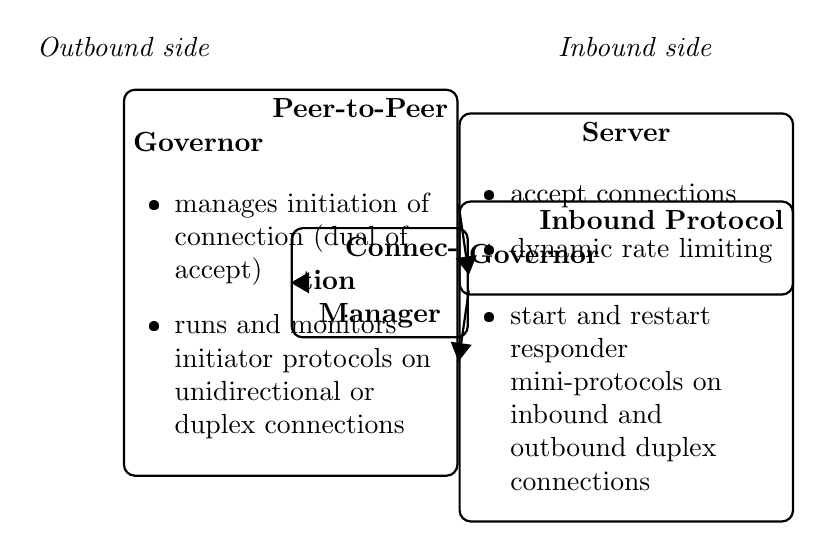
\begin{tikzpicture}
    \node at (-3.25, 0)  {\textit{Outbound side}};
    \node at ( 3.25, 0)  {\textit{Inbound side}};

    \node[rounded corners, rectangle, draw, minimum height=3cm,anchor=east, text width=4cm] (p2p_governor) at (\xa, -3)
     {
       \hfil\textbf{Peer-to-Peer Governor}\hfil\\
       \setlength{\leftmargini}{15pt}
       \begin{itemize}
        \item manages initiation of connection (dual of accept)
        \item runs and monitors initiator protocols on unidirectional or duplex connections
      \end{itemize}
      \vspace{5pt}
      };

    \node[rounded corners, rectangle, draw, anchor=west, text width=4cm] (server) at (\xb, -2)
      {
        \hfill{\textbf{Server}}\hfill
        \vspace{0.2em}
        \setlength{\leftmargini}{15pt}
        \begin{itemize}
          \item accept connections
          \item dynamic rate limiting
        \end{itemize}
        \vspace{5pt}
      };

    \node[rounded corners, rectangle, draw, anchor=west, text width=4cm] (inbound_governor) at (\xb, -4)
      {
        \hfill{\textbf{Inbound Protocol Governor}}\hfill
        \vspace{0.2em}
        \setlength{\leftmargini}{15pt}
        \begin{itemize}
          \item start and restart responder mini-protocols on inbound and
            outbound duplex connections
        \end{itemize}
        \vspace{5pt}
      };

    \node[rounded corners, rectangle, draw, minimum height=1cm, text width=2cm] (connection_manager) at (0, -3)
      {
        \hfil\textbf{Connection}\hfil\\
        \hfil\textbf{Manager}\hfil
      };

    \draw[<-] (p2p_governor)           -- (connection_manager);
    \draw[->] (server.west)            -- (connection_manager.5);
    \draw[->] (connection_manager.355) -- (inbound_governor.west);
  \end{tikzpicture}
\end{figure}

\section{Connection Manager}

\Connmngr{} exposes two methods to register a connection:
\begin{lstlisting}
data Connected peerAddr handle handleError
  -- | We are connected and mux is running.
  = Connected    !(ConnectionId peerAddr) !handle

  -- | There was an error during handshake negotiation.
  | Disconnected !(ConnectionId peerAddr) !(Maybe handleError)

-- | Include outbound connection into 'ConnectionManager'.
requestOutboundConnection
  *'$\coloncolon$'* HasInitiator muxMode ~ True
  *'$\Rightarrow$'* ConnectionManager muxMode socket peerAddr handle handleError m
  *'$\rightarrow$'* peerAddr *'$\rightarrow$'* m (Connected peerAddr handle handleError)

-- | Include an inbound connection into 'ConnectionManager'.
includeInboundConnection
  *'$\coloncolon$'* HasResponder muxMode ~ True
  *'$\Rightarrow$'* ConnectionManager muxMode socket peerAddr handle handleError m
  *'$\rightarrow$'* socket *'$\rightarrow$'* peerAddr *'$\rightarrow$'* m (Connected peerAddr handle handleError)
\end{lstlisting}
The first one asks the \connmngr{} to either connect a peer or if
possible reuse a duplex connection.  The other one allows to register an
inbound connection, which was \texttt{accepted}.  Both methods are blocking
operations and return either an error (handshake negotiation error or
a multiplexer error) or a handle to a \textit{negotiated} connection.

Other methods which are discussed in this specification:

\begin{lstlisting}
-- | Custom either type for result of various methods.
data OperationResult a
    = UnsupportedState !InState
    | OperationSuccess a


-- | Enumeration of states, used for reporting; constructors elided from this
-- specification.
data InState

-- | Unregister an oubound connection.
-- 
unregisterOutboundConnection
  *'$\coloncolon$'* HasInitiator muxMode ~ True
  *'$\Rightarrow$'* ConnectionManager muxMode socket peerAddr handle handleError m
  *'$\rightarrow$'* peerAddr *'$\rightarrow$'* m (OperationResult ())

-- | Notify the 'ConnectionManager' that the remote end promoted us to a /warm
-- peer/; this runs the @PromotedToWarm^{duplex}_{remote}@ transition.
promotedToWarmRemote
  *'$\coloncolon$'* HasInitiator muxMode ~ True
  *'$\Rightarrow$'* ConnectionManager muxMode socket peerAddr handle handleError m
  *'$\rightarrow$'* peerAddr *'$\rightarrow$'* m (OperationResult ())

-- | Unregister outbound connection.  Returns if the operation was successul.
unregisterInboundConnection
  *'$\coloncolon$'* HasResponder muxMode ~ True
  *'$\Rightarrow$'* ConnectionManager muxMode socket peerAddr handle handleError m
  *'$\rightarrow$'* peerAddr *'$\rightarrow$'* m (OperationResult Bool)

-- | Number of connections tracked by the server.
numberOfConnections
  *'$\coloncolon$'* HasResponder muxMode ~ True
  *'$\Rightarrow$'* ConnectionManager muxMode socket peerAddr handle handleError m
  *'$\rightarrow$'* STM m Int
\end{lstlisting}

\section{Connection states}

Each connection is either initiated by \texttt{Inbound} or \texttt{Outbound} side.
\begin{lstlisting}
data Provenance
  = Inbound
  | Outbound
\end{lstlisting}
Each connection negotiates \texttt{dataFlow}:
\begin{lstlisting}
data DataFlow
  = Unidirectional
  | Duplex
\end{lstlisting}
Negotiation of \texttt{DataFlow} is done by the handshake protocol, the final
result depends on two factors: negotiated version and \texttt{InitiatorOnly}
flag which is announced through handshake.  Each connection can be in one
of the following states:
\begin{lstlisting}
data ConnectionState
  -- Connection manger is about to connect to a peer.
  = ReservedOutboundState

  -- Connected to a peer, handshake negotiation is ongoing.
  | UnnegotiatedState Provenance

  -- Inbound connection has been negotiated.
  | InboundState DataFlow

  -- Outbound connection has been negotiated.
  | OutboundState DataFlow

  -- Connection runs in duplex mode: either outbound connection negotiated
  -- 'Duplex' data flow, or 'InboundState Duplex' was reused.
  | DuplexState

  -- Connection has terminated; socket is released, thread running the
  -- connection is closed.  For some small delay the connection is kept in this
  -- state until the kernel releases all the resources.
  | TerminatingState

  -- Connection is removed from connection manager map, at this point the
  -- connection manager can create a new connection to that peer.
  | TerminatedState
\end{lstlisting}
The above type is a stripped version of what is implemented.  The real
implementation tracks more detail, e.g. connection id (the quadruple of ip
addresses and ports), multiplexer handle, etc.

\begin{figure}[p]
  {\hspace{-3cm}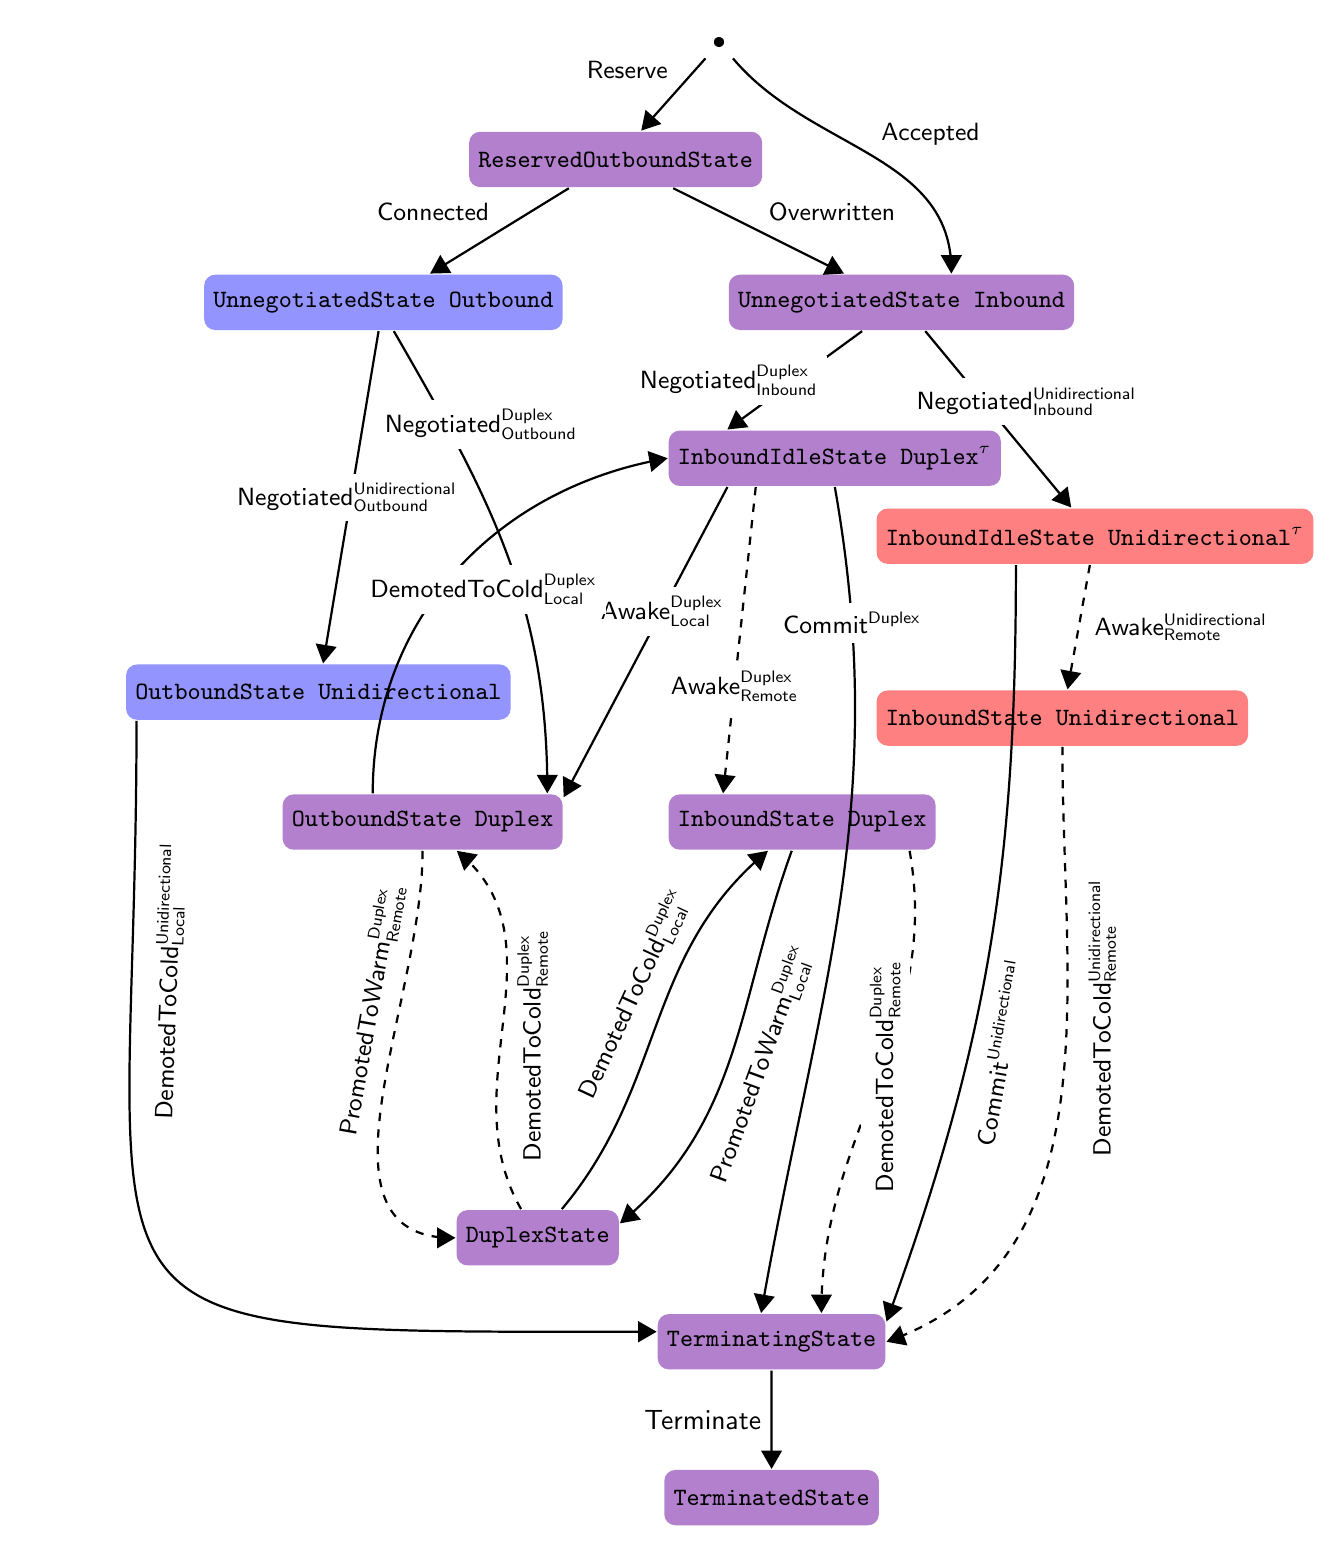
\begin{tikzpicture}[scale=0.66]
    \node                         (init)                               at ( 2,   2)     {\small\InitialState};
    \node[inbound_outbound_state] (ReservedOutboundState)              at ( 0,-0.25)    {\small\ReservedOutboundState};
    \node[outbound_state,anchor=east] (UnnegotiatedState_Outbound)     at (-1,  -3)     {\small\UnnegotiatedStateOut};
    \node[inbound_outbound_state] (UnnegotiatedState_Inbound)          at ( 5.5, -3)    {\small\UnnegotiatedStateIn};
    \node[inbound_outbound_state,anchor=west] (InboundIdleState_DupDF)    at ( 1, -6.0) {\small\InboundIdleStateDupStar};
    \node[inbound_state,anchor=west] (InboundIdleState_UniDF)             at ( 5, -7.5) {\small\InboundIdleStateUniStar};
    \node[outbound_state,anchor=east]            (OutboundState_UniDF) at (-2, -10.5)   {\small\OutboundStateUni};
    \node[inbound_outbound_state,anchor=east]    (OutboundState_DupDF) at (-1,  -13)    {\small\OutboundStateDup};
    \node[inbound_state,anchor=west] (InboundState_UniDF)              at ( 5, -11)     {\small\InboundStateUni};
    \node[inbound_outbound_state,anchor=west] (InboundState_DupDF)     at ( 1,  -13)    {\small\InboundStateDup};
    \node[inbound_outbound_state] (DuplexState)                        at (-1.5, -21)   {\small\DuplexState};
    \node[inbound_outbound_state] (TerminatingState)                   at ( 3,  -23)    {\small\TerminatingState};
    \node[inbound_outbound_state] (TerminatedState)                    at ( 3,  -26)    {\small\TerminatedState};


    \draw[->] (init) -- node[fill=white,pos=0.425,above left]{\small\Reserve}                                       (ReservedOutboundState);
    \draw[->] (init) to [out=310, in=90] node[fill=white, above right]{\small\Accepted}                             (UnnegotiatedState_Inbound.30);

    \draw[->] (ReservedOutboundState)          -- node[fill=white,above left] {\small\Connected}                    (UnnegotiatedState_Outbound);
    \draw[->] (ReservedOutboundState)          -- node[fill=white,above right] {\small\Overwritten}                 (UnnegotiatedState_Inbound);

    \draw[->] (UnnegotiatedState_Outbound)     -- node[fill=white,left=-42pt] {\small\NegotiatedUniOut}             (OutboundState_UniDF);
    \draw[->] (UnnegotiatedState_Outbound.290) to [out=-60, in=90]
                                                  node[fill=white,right=-26pt,pos=0.2]{\small\NegotiatedDupOut}     (OutboundState_DupDF.13);

    \draw[->] (UnnegotiatedState_Inbound)          -- node[fill=white,left=-12pt]{\small\NegotiatedDupIn}           (InboundIdleState_DupDF.165);
    \draw[->] (UnnegotiatedState_Inbound)          -- node[fill=white,pos=0.4,right=-28pt]{\small\NegotiatedUniIn}  (InboundIdleState_UniDF);
    \draw[->, dashed] (InboundIdleState_UniDF) -- node[fill=white,right=2pt]{\small\AwakeUniRem}                    (InboundState_UniDF);

    \draw[->, dashed] (InboundState_UniDF) to [out=270, in=20]  node[right=20pt,rotate=90,pos=0.6]{\small\DemotedToColdUniRem}    (TerminatingState.0);
    \draw[->, dashed] (InboundState_DupDF.345) to [out=280, in=90]  node[fill=white,left=10pt,rotate=90,pos=0.2]{\small\DemotedToColdDupRem}
                                                                                                                                  (TerminatingState.30);
    \draw[->]         (InboundIdleState_DupDF.195) -- node[fill=white,pos=0.4]{\small\AwakeDupLoc}                                (OutboundState_DupDF.10);

    \draw[->, dashed] (InboundIdleState_DupDF.200) -- node[fill=white,pos=0.65]{\small\AwakeDupRem}                                           (InboundState_DupDF.160);
    \draw[->]         (OutboundState_DupDF.150) to [out=90,in=-170] node[fill=white,pos=0.45,left=-60pt]{\small\DemotedToColdDupLoc}          (InboundIdleState_DupDF.180);
    \draw[->]         (DuplexState)             to [out=50,in=220]  node[fill=white,pos=0.90,left=18pt,rotate=65]{\small\DemotedToColdDupLoc} (InboundState_DupDF);
    \draw[->]         (InboundState_DupDF)      to [out=-110,in=40] node[pos=0.9,right=22pt,rotate=70]{\small\PromotedToWarmDupLoc}           (DuplexState.10);
    \draw[->, dashed] (DuplexState)             to [out=120,in=-40] node[fill=white,right=10pt,pos=0.1,rotate=90]{\small\DemotedToColdDupRem} (OutboundState_DupDF);
    \draw[->, dashed] (OutboundState_DupDF)     to [out=-90,in=180] node[left,pos=0.05,left=10pt,rotate=80]{\small\PromotedToWarmDupRem}      (DuplexState);

    \draw[->]         (InboundIdleState_DupDF.270) to[out=-80,in=80] node[fill=white,pos=0.15]{\small\CommitDup}                              (TerminatingState.110);
    \draw[->]         (InboundIdleState_UniDF.200) to[out=-90,in=70] node[fill=white,pos=0.5,rotate=80,left=-10pt]{\small\CommitUni}          (TerminatingState.10);

    \draw[->] (OutboundState_UniDF.189)        to [out=270, in=180,pos=0.23,looseness=2]
                                                  node[right=12pt,rotate=88,pos=0.3]{\small\DemotedToColdUniLoc} (TerminatingState.175);

    \draw[->] (TerminatingState) -- node[left]{\Terminate} (TerminatedState);
  \end{tikzpicture}}
  \caption{\textit{Outbound} (blue \& violet) and \textit{inbound} (red \&
  violet) connection states and allowed transitions.  Dashed arrows indicate an
  asynchronous transition, either driven by the decision of a remote peer
  (\DemotedToColdUniRem{} and \DemotedToColdDupRem{}) or the local \connmngr{}
  itself. States which are decorated with $^\tau$ have an associated timeout,
  see~\ref{sec:tr_commit}.}
  \label{fig:statediagram}
\end{figure}

Figure~\ref{fig:statediagram} shows all the transitions between
\texttt{ConnectionState}s.  Blue and violet states represent states of
an \textit{outbound} connection, red and violet represent states of an
\textit{inbound} connection.  Dashed arrows indicate an asynchronous
transitions that are triggered either by remote node or by the connection
manger itself.

Note that the vertical symmetry in the graph corresponds to local / remote
state of the connection:

\begin{table}[h]
  \begin{tabular}[h]{l|l}
    \textit{local connection state} & \textit{remote connection state} \\ [0.3em]
    \hline \\ 
    \UnnegotiatedStateOut{}         & \UnnegotiatedStateIn{}           \\ [0.2em]
    \OutboundStateAny{}             & \InboundStateAny{}               \\ [0.2em]
    \InboundStateAny{}              & \OutboundStateAny{}              \\ [0.2em]
    \DuplexState{}                  & \DuplexState{}                   \\ [0.2em]
  \end{tabular}
\end{table}


\section{Transitions}

\subsection{\Reserve{}}
When \connmngr{} is asked for an outbound connection, it reserves a slot
in its state for that connection.  If any other thread will ask for the same
outbound connection, the \connmngr{} will raise an exception in that thread.
Reservation is done to guarantee exclusiveness for state transitions to
a single outbound thread.

\subsection{\Connected{}}
This transition is executed once an outbound connection successfully performed
\texttt{connect} system call. 

\subsection{\Accepted{} and \Overwritten{}}
Transition driven by \texttt{accept} system call.  Once it returns the
\connmngr{} might either not know about such connection or be in
\ReservedOutboundState{}.  \Accepted{} transition represents the former
situation while the latter is captured by \Overwritten{} transition.

Let us note that if \Overwritten{} transition happened, then on the outbound
side the scheduled \texttt{connect} call will fail.  In this case the
\ptopgov{} will recover, put the peer in a queue of failed peers, and
will either try to connect to another peer or reconnect to that peer after some
delay in which case it would re-use the accepted connection (assuming that
duplex connection was negotiated).

\subsection{\NegotiatedUniOut{} and \NegotiatedDupOut{}}
Once an outbound connection has been negotiated one of \NegotiatedUniOut{} or
\NegotiatedDupOut{} is performed, depending on the result of handshake
negotiation.  Duplex connections are negotiated only for node-to-node protocol
version higher than \texttt{NodeToNodeV\_7}\todoimpl{the exact version number
mightchange} and neither side declared that it is an initiator only.

If duplex outbound connection was negotiated, the \connmngr{} needs to ask the
\inbgov{} to start and monitor responder mini-protocols on the outbound
connection.

This transition is done by the \texttt{requestOutboundConnection}.

\subsection{\NegotiatedUniIn{} and \NegotiatedDupIn{}}
This transition is performed once handshake negotiated a unidirectional or
duplex connection on an inbound connection.  The \textit{inbound protocol
governor} will start all responder protocols (for all \established{}, \warm{}
and \hot{} groups of mini-protocols) and keep monitoring them.

This transition is done by the \texttt{includeInboundConnection}.

\subsection{\AwakeDupLoc{}, \AwakeDupRem{} and \AwakeUniRem{}}
All the awake transitions start either at \InboundIdleStateUni{} or
\InboundIdleStateDup{}.  \AwakeDupRem{} and \AwakeUniRem{} are triggered by
incomming traffic on any of the responders. \AwakeDupLoc{} transition however
is done by \texttt{requestOutboundConnection} on request of \ptopgov{}.

\subsection{\CommitUni{}, \CommitDup{}}\label{sec:tr_commit}
Both commit transition happen after a timeout of inactivity.  They transition
to \TerminatingState{} (closing the bearer).  For duplex connections a normal
shutdown procedure goes through \InboundStateDup{} via \CommitDup{} - which
gave the name to this transitions.

\subsection{\DemotedToColdUniLoc{}}
This transition is driven by the \ptopgov{}: when it decides to demote the peer
to \cold{} state.  This transition should trigger a normal \TCP{} termination,
via \texttt{close} call: we started the connection, and thus we are in position
to close it.

This transition is realised by \texttt{unregisterOutboundConnection}.

\subsection{\DemotedToColdDupLoc{}}
As above this transition is driven by the local \ptopgov{}, but this time it is
triggered on a connection in \texttt{DuplexState}.  The \connmngr{} will need
to be instructed to change the connection state.

This transition is realised by \texttt{unregisterOutboundConnection}.

\subsection{\PromotedToWarmDupLoc{}}
This transition is driven by the local \ptopgov{} when it promotes a \cold{} peer
to \warm{} state.  This is the case where a \connmngr{} will provide
a handle to an existing connection to the \ptopgov{}.

This transition is realised by \texttt{requestOutboundConnection}.

\subsection{\DemotedToColdUniRem{}, \DemotedToColdDupRem{}}
The \DemotedToColdUniRem{} and the two \DemotedToColdDupRem{} transitions are triggered
when the remote end demotes the local peer to \cold{}.  The \inbgov{} can
notice this when one of the \established{} protocols returns.  It will need to
inform the \connmngr{} that this transition happened.  For the
\DemotedToColdDupRem{} from \InboundStateDup{} there is a potential race
condition on which side will call \texttt{close} first.  For this reason it is
safer to transition to \TerminatingState{}.  For \DemotedToColdUniRem{} we
expect that the remote side will call \texttt{close} as soon as it terminated
all its \established{} mini-protocols.  In this case We transition to
\TerminatingState{}.  Even though it's expected that the remote side, which
initiated the connection, calls close first we simply cannot assume
that.  It's not unlikely that both sides will do simultanous \TCP{} close.
Also even if the remote and ended up in \texttt{TIME\_WAIT} state not us,
re-establishing a \TCP{} connection relies on the initial sequence number of
the new connection to be larger than the previous connection (see~\cite[Chapter
2, \texttt{TIME\_WAIT} section]{stevens2003unix}, \cite[Section
4.2.2.13]{RFC1122}), a property we don't want to relay on (various
implementations might vary). For all these reasons transition to
\TerminatingState{,} which will hold the connection for \texttt{TIME\_WAIT}
interval, is a safer option.

This transitions are realised by \texttt{unregisterInboundConnection}.

\subsubsection{Restarting a mini-protocol}
When the server restarts a responder side of a mini-protocol is not a visible
state transition to the governor but it deserves to be described.  The actions
depend on the state in which is the connection:

\paragraph{\DuplexState{}:}
if any responder side of a mini-protocol returns, we
restart it.  This must be a result of either \warm{} to \hot{}, \hot{} to
\warm{} or a transition to \cold{}.  In \DuplexState{} we don't need to
distinguish them: in either case the local \ptopgov{} is still using this
connection.  Note that even in the case of being demoted to \cold{} (and thus
executing \DemotedToColdDupRem{} transition), we restart all the
mini-protocols.

\paragraph{\InboundStateAny{}:}
in these states we need to distinguish remote transtions between \warm{} and
\hot{} and transtions to \cold{}.  In the latter case a mini-protocol shall be
restarted, in the former the \inbgov{} needs to trigger termination procedure:
await with a timeout for all mini-protocols to terminate, when that happens
check once again whether connection is not in \DuplexState{} and trigger one of
\DemotedToColdDupRem{} or \DemotedToColdUniRem{} transition.

We can distinguish transition remote transitions to \cold{} state from
transitions between \warm{} and \hot{} states simply by noticing that an
\established{} mini-protocol terminated.

This transition is implemented with the help of \texttt{isInDuplexState}.

\subsection{\PromotedToWarmDupRem{}}
This transition is triggered by the remote peer, and thus is asynchronous.  The
\inbgov{} can notice it by observing multiplexer ingress side of \established{}
mini-protocols.\footnote{The \texttt{network-mux} library allows to start
mini-protocols lazily, as soon a message for the given mini-protocol is
registered by demultiplexer. For the lazily started mini-protocols the
transtion from \texttt{StatusStartOnDemand} to \texttt{StatusRunning} captures
the state change we are looking for in \PromotedToWarmDupRem{} transition.}
It then should notfiy the \connmngr{}.

This transitions are realised by \texttt{promotedToWarmRemote}.

\subsection{\Prune{} transitions}
First let us note that a connection in \InboundStateDup{}, could have been
initiated by either side.  This means that even though a node might have not
accepted any connection it could end up serving peers and possible go beyond
server hard limit and thus exceed the number of file descriptors.  This is
thanks to the path:
\begin{itemize}
  \item[] \Connected{},
  \item[] \NegotiatedDupOut{},
  \item[] \PromotedToWarmDupRem{},
  \item[] \DemotedToColdDupLoc{}
\end{itemize}
which leads from the initial state \InitialState{} to \InboundStateDup{}, the
same state in which accepted duplex connections end up.  Even though the server
rate limits connections based on how many connections are in this state, we
could end up exceeding server hard limit.

To solve this problem, when a connection is transitioned from 
\DuplexState{} to \InboundStateDup{} (via \DemotedToColdDupLoc{}) the
\connmngr{} will check if we the server hard limit was exceeded.  If that
happened, the \connmngr{} will reset a connection.

If we keep the number of \established{} peers to be smaller than the server
hard limit, we should never need to reset a connection in \DuplexState{}.

We prefer to reset an inbound connections rather than close an outbound
connection because from systemic point of view, outbound connections are more
valuable than inbound ones.

The \textit{inbound protocol governor} is in position to make an educated
decision which connection to reset.  Initially, we aim for a decision driven by
randomness, but other choices are possible\footnote{We can take into account
whether we are \hot{} to the remote end, or for how long we have been \hot{} to
to the remote node.} and the implementation should allow to easily extend the
initial choice.

\subsection{\TerminatingState{} and \TerminatedState{}}
After a connection was closed we keep it in \TerminatingState{} for some time.
This allows for the kernel to release all the resources (addresses).  After
this fixed timeout the connection is removed from the \connmngr{} state,
which we explicitely signify in this specification as \TerminatedState{}.

From operational point of view it's important that connections are not held in
\texttt{TIME\_WAIT} state for too long.  This would be problematic when
restarting a node (without rebooting the system) (e.g. when adjusting
configuration).  The \connmngr{} makes sure that it closes outbound
connections as soon as it can, which means it will only held its outbound
connections in \texttt{TIME\_WAIT} state.  The system setting for
\texttt{TIME\_WAIT} delay is well designed for various network conditions, for
example on Linux it is \texttt{60s}.  To avoid this problem for local relays,
the \connmngr{} can be configured to use ephemeral port for specific
outbound connections.

\subsection{Protocol errors}
If a mini-protocol errors, on either side, connection will be reset (as opposed
to \texttt{close}), and put in \TerminatedState{}.  This can possibly happen in
any connection state.

{\small
Note for implementation: reseting conndtion should be the default.  It can be
set with \texttt{SO\_LINGER} option with a zero linger interval.  This will
cause \texttt{close} call to include \texttt{RST} \TCP{} header.  There are
only two cases where we need \texttt{close} rather than \texttt{reset}:
\DemotedToColdUniLoc{} and \DemotedToColdDupLoc{}.
}

\section{\textit{Outbound} connection}

The state of a connection when \texttt{includeoutboundConnection} is called
which leads to either \OutboundStateUni{} or \DuplexState{} must be either:
\ReservedOutboundState{}, \UnnegotiatedStateIn{} or
\InboundStateDup{}.  If the initial state is \UnnegotiatedStateIn{} then the
the result depends on the negotiation.  If \texttt{Unidirectional} connection was
negotiated \texttt{includeoutboundConnection} must error, if \texttt{Duplex}
connection was negotiated it can use the egress side of this connection leading
to \DuplexState{}.

\paragraph{\textnormal{initial state (\InitialState{})}:} the \connmngr{} does not have
  a connection with that peer.  The  connection is put \ReservedOutboundState{}
  before \connmngr{} connects to that peer;

\paragraph{\UnnegotiatedStateIn{}:} if the \connmngr{} accepted
  a connection from that peer, handshake is ongoing;
  \texttt{requestOutboundConnection} will await until the connection state
  changes to \InboundStateAny{}.

\paragraph{\InboundStateUni{}:} if \texttt{requestOutboundConnection} finds
a connection in this state it will error.

\paragraph{\InboundStateDup{}:} if \connmngr{} accepted connection from
  that peer and handshake negotiated a \texttt{Duplex} data flow;

\paragraph{\TerminatingState{}:} block until \TerminatedState{} and start from
the initial state.

\paragraph{\textnormal{Otherwise}:} if \connmngr{} is asked to connect to
peer and there exists a connection which is in any other state, e.g.
\UnnegotiatedStateOut{}, \OutboundStateAny{}, \DuplexState{}, \connmngr{} signals the caller with an error, see
section~\ref{sub:includeOutboundConnect}.

Figure~\ref{fig:outbound_flow} shows outbound connection state evolution.  This
shows the exact steps and decisions that \texttt{requestOutboundConnection}
needs to make.

\begin{figure}[p]
  \footnotesize{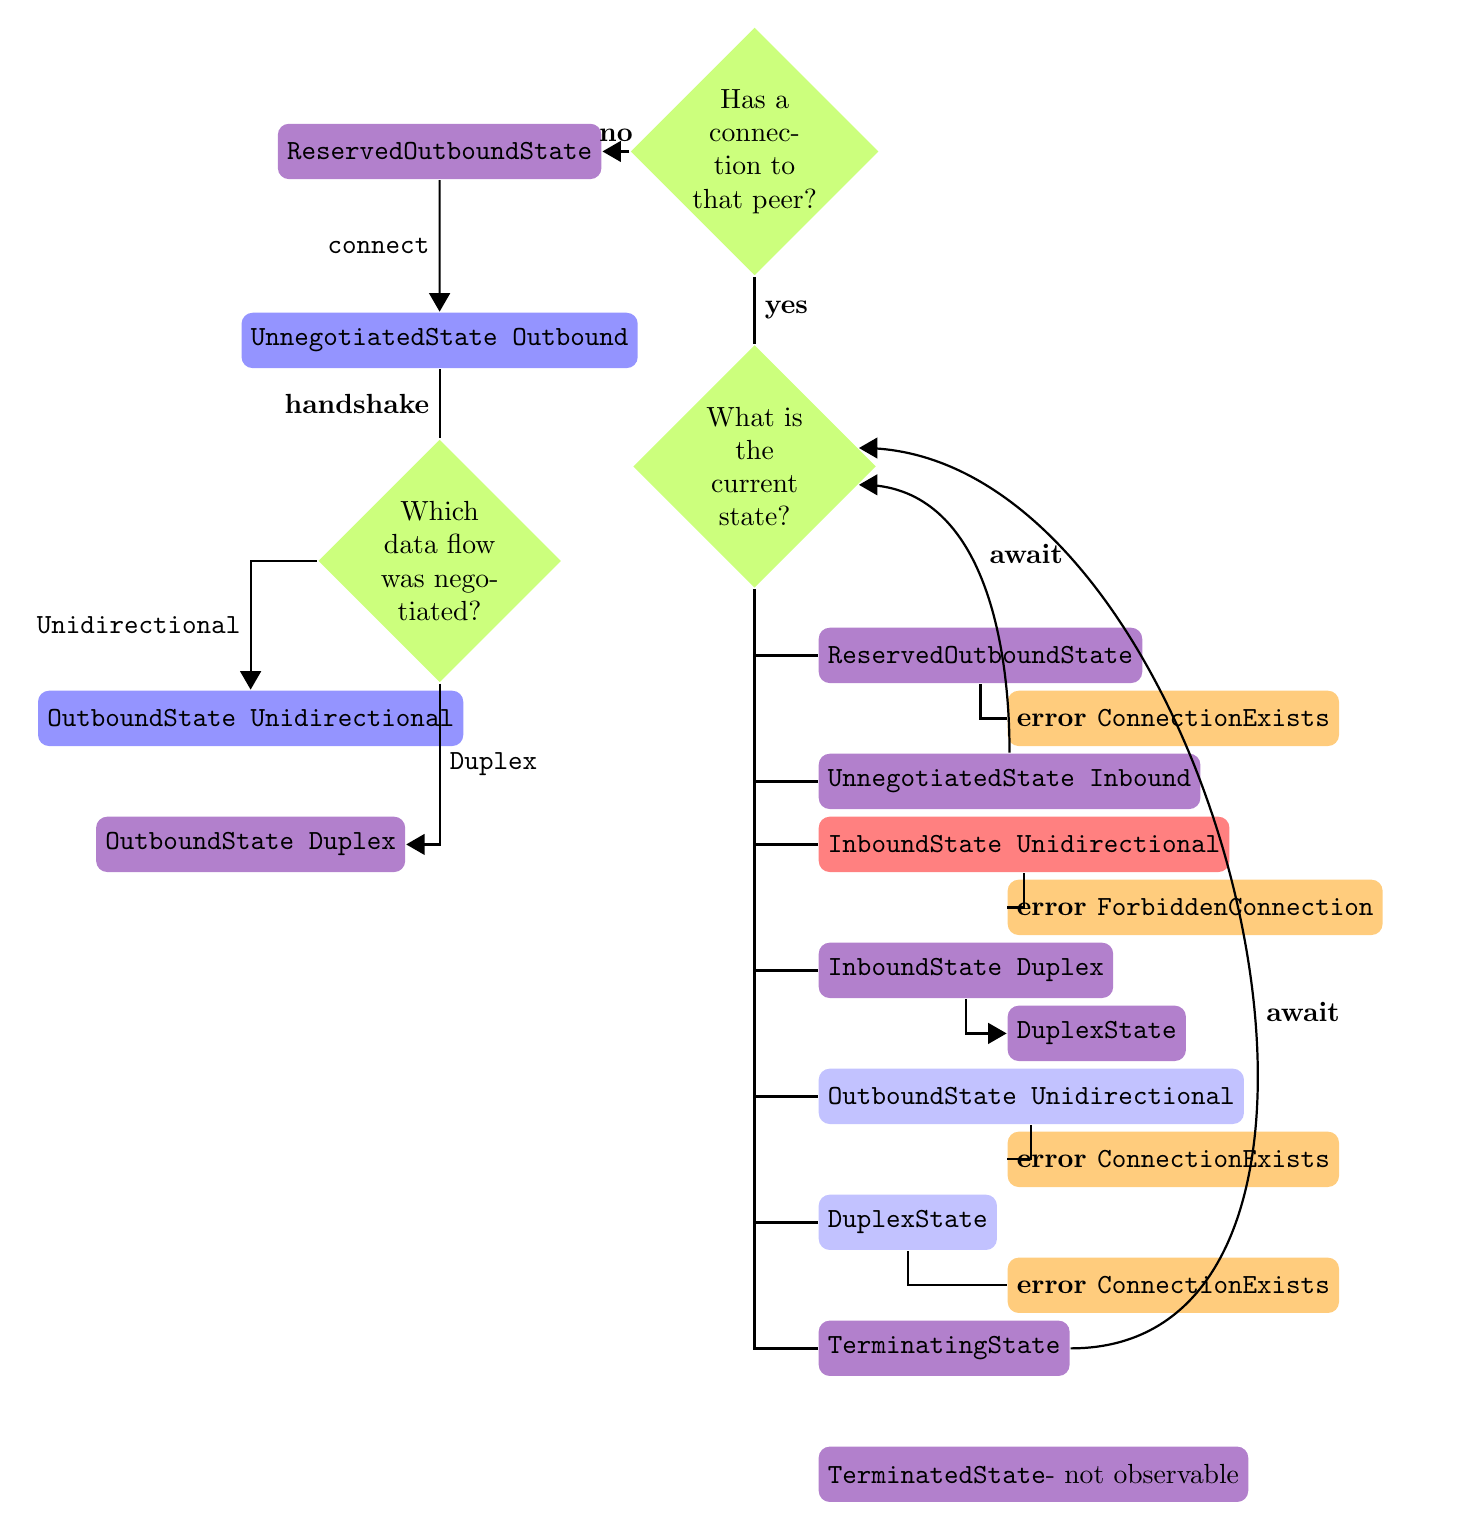
\begin{tikzpicture}[scale=0.8]
    \node[decision]               (init)      at (0,0) {Has a connection to that peer?};
    \node[inbound_outbound_state] (not_found) at (-5, 0) {\ReservedOutboundState{}};

    % Connection not found flow
    \draw[->] (init) -- node[above] {\textbf{no}}  (not_found);
    \node[outbound_state] (connected) at (-5, -3) {\UnnegotiatedStateOut{}};
    \draw[->] (not_found) -- node[left] {\textbf{\texttt{connect}}} (connected);

    % This may be influenced by `initiator only` flag or version of the connection.
    \node[decision]               (handshake_decision_outbound) at (-5, -6.5) {Which data flow was negotiated?};
    \node[outbound_state]         (outbound_unidf)              at (-8, -9)   {\OutboundStateUni{}};
    \draw (connected) -- node[left] {\textbf{\textbf{handshake}}} (handshake_decision_outbound);

    \node[inbound_outbound_state] (outbound_dupdf)             at (-8, -11)  {\OutboundStateDup{}};
    \draw[->] (handshake_decision_outbound.west) -| node[left, near end] {\texttt{Unidirectional}} (outbound_unidf);
    \draw[->] (handshake_decision_outbound) |- node[right, near start] {\textbf{\texttt{Duplex}}} (outbound_dupdf);

    % Connection found flow

    \node[decision] (found) at (0, -5)     {What is the current state?};
    \draw (init) -- node[right] {\textbf{yes}} (found);

    \node[inbound_outbound_state,anchor=west] (reserved_outbound) at (1, -8)  {\ReservedOutboundState};
    \node[error,anchor=west]                  (termination_c)     at (4, -9) {\textbf{error \texttt{ConnectionExists}}};
    \draw   (found.south)       |- (reserved_outbound);
    \draw[] (reserved_outbound) |- (termination_c);

    \node[inbound_outbound_state,anchor=west] (unnegotiated_inbound) at (1, -10) {\UnnegotiatedStateIn};
    \draw (found.south) |- (unnegotiated_inbound.west);
    \draw[->] (unnegotiated_inbound) to[out=90,in=0] node[above right] {\textbf{await}} (found.350);

    \node[inbound_state,anchor=west] (inbound_unidf) at (1, -11) {\InboundStateUni};
    \node[error,anchor=west] (termination_unidf) at (4, -12) {\textbf{error \texttt{ForbiddenConnection}}};
    \draw (found.south) |- (inbound_unidf);
    \draw[] (inbound_unidf) |- (termination_unidf);

    \node[inbound_outbound_state,anchor=west] (inbound_dupdf) at (1, -13) {\InboundStateDup};
    \node[inbound_outbound_state,anchor=west] (duplex)        at (4, -14) {\DuplexState};
    \draw (found.south) |- (inbound_dupdf);
    \draw[->] (inbound_dupdf) |- (duplex);


    \node[impossible_outbound_state,anchor=west] (outbound_uni) at (1, -15) {\OutboundStateUni};
    \draw (found.south) |- (outbound_uni);
    \node[error,anchor=west] (termination_outuni) at (4, -16) {\textbf{error \texttt{ConnectionExists}}};
    \draw (outbound_uni) |- (termination_outuni.west);

    \node[impossible_outbound_state,anchor=west] (duplex_imp)   at (1, -17) {\DuplexState};
    \draw (found.south) |- (duplex_imp);
    \node[error,anchor=west] (termination_dupuni) at (4, -18) {\textbf{error \texttt{ConnectionExists}}};
    \draw (duplex_imp) |- (termination_dupuni.west);

    \node[inbound_outbound_state,anchor=west] (terminating) at (1, -19) {\TerminatingState};
    \draw (found.south) |- (terminating);
    \draw[->] (terminating.0) to [out=0,in=0] node[above right,pos=0.4] {\textbf{await}} (found.10);

    \node[inbound_outbound_state,anchor=west] (terminated)  at (1, -21) {\TerminatedState - not observable};

  \end{tikzpicture}}
  \caption{\textit{Outbound} connection flow graph}
  \label{fig:outbound_flow}
\end{figure}

\subsection{\OutboundStateDup{} and \DuplexState{}}
Once an outbound connection negotiates \texttt{Duplex} data flow it transfers
to \OutboundStateDup{}.  At this point we need to start responder protocols.
This means that the \connmngr{} needs a way to inform server (which
accepts and monitors inbound connections), to start the protocols and monitor
that connection.  This connection will transitioned to \DuplexState{} only once
we notice incoming traffic on any of \established{} protocols.

The implementation is using
\href{https://github.com/input-output-hk/ouroboros-network/blob/coot/connection-manager/ouroboros-network-framework/src/Ouroboros/Network/ConnectionManager/Server/ControlChannel.hs\#L123}{\texttt{TBQueue}}.
Server is using this channel for monitoring inbound connections which includes
starting responder protocols.

\subsection{Termination}\label{sec:outbound_termination}

When \ptopgov{} demotes a peer to \cold{} state an outbound
connection needs to transition either from \OutboundStateUni{} to
\TerminatingState{} or from \DuplexState{} to \InboundStateDup{}.  To
support that the \connmngr{} exposes a method:
\begin{lstlisting}
unregisterOutboundConnection *'$\coloncolon$'* peerAddr *'$\rightarrow$'* m ()
\end{lstlisting}
This method performs \DemotedToColdUniLoc{} or
\DemotedToColdDupLoc{} transition. In the former case it will shut down the
multiplexer and close the \TCP{} connection, in the latter case, beside
changing the connection state, it will also trigger \Prune{} transitions if
the number of inbound connections becomes above the limit.

\subsection{Connection manager methods}
\subsubsection{\texttt{requestOutboundConnection}}\label{sub:includeOutboundConnect}
\begin{tabular}[h]{ll}
  \textit{State}           & \textit{Action} \\\hline\\[2pt]
  \InitialState{}          &
    \begin{minipage}[t]{8cm}
      \begin{itemize}
        \item \ReservedOutboundState{},
        \item \Connected{},
        \item start connection thread (handshake, \mux{})
        \item \NegotiatedUniOut{} or \NegotiatedDupOut{}
      \end{itemize}
    \end{minipage}
    \vspace{8pt}\\
  \ReservedOutboundState{} & error \texttt{ConnectionExists} \\[8pt]
  \UnnegotiatedStateOut{}  & error \texttt{ConnectionExists} \\[8pt]
  \UnnegotiatedStateIn{  } &
    \begin{minipage}[t]{7cm}
      await for \InboundStateAny{}, if negotiated duplex connection
      transition to \DuplexState{}, otherwise error
      \texttt{ForbiddenConnection}
    \end{minipage}
    \vspace{8pt}\\
  \OutboundStateAny{}      & error \texttt{ConnectionExists} \\[8pt]
  \DuplexState{}           & error \texttt{ConnectionExists} \\[8pt]
  \TerminatingState{}      & await for \TerminatedState{}    \\[8pt]
  \TerminatedState{}       & can be treated as initial state \\[8pt]
\end{tabular}

\subsection{\texttt{unregisterOutboundConnection}}
\begin{tabular}[h]{ll}
  \textit{State}           & \textit{Action} \\\hline\\[2pt]
  \InitialState{}          & \texttt{no-op} \\[8pt]
  \ReservedOutboundState{} & error \texttt{ForbiddenOperation} \\[8pt]
  \UnnegotiatedStateOut{}  & error \texttt{ForbiddenOperation} \\[8pt]
  \UnnegotiatedStateIn{}   & error \texttt{ForbiddenOperation} \\[8pt]
  \OutboundStateUni{}      & \DemotedToColdUniLoc{} \\[8pt]
  \OutboundStateDup{}      & \DemotedToColdDupLoc{} \\[8pt]
  \DuplexState{}           & prune connections and run \DemotedToColdDupLoc{} \\[8pt]
  \TerminatingState{}      & \texttt{no-op} \\[8pt]
  \TerminatedState{}       & \texttt{no-op} \\[8pt]
\end{tabular}
The choice between \texttt{no-op} and error is solved by the followin rule: if
the calling component (e.g. \ptopgov{}), is able to keep its state in
a consistent state with \connmngr{} then use \texttt{no-op}, otherwise
error.  Since both \inbgov{} and \ptopgov{} are using \mux{} to track the state
of the connection its actually impossible that the state would be inconsistent.

\section{\textit{Inbound} connection}
Initial states for inbound connection is either:
\begin{itemize}
  \item The initial state: \InitialState{};
  \item \ReservedOutboundState{}
    This can happen when
    \begin{center}
      \texttt{requestOutboundConnection}
    \end{center}
    reserves a connection with \ReservedOutboundState{}, but before it calls
    \texttt{connect} the \texttt{accept} call returned.  In this case, the
    \texttt{connect} call will fail and, as a consequence,
    \texttt{requestOutboundConnection} will fail too.  Any mutable variables
    used by it can be disposed, since there is no thread that could be blocked
    on it: if there was another thread that asked for an oubound connection
    with that peer it would see \ReservedOutboundState{} and it throw
    \texttt{ConnectionExists} exception.

    To make sure that this case is uncommon, we need to guarantee that the
    \connmngr{} does not block between putting the connection in the
    \ReservedOutboundState{} and calling the \texttt{connect} system call.
\end{itemize}

\begin{figure}[h]
  \footnotesize{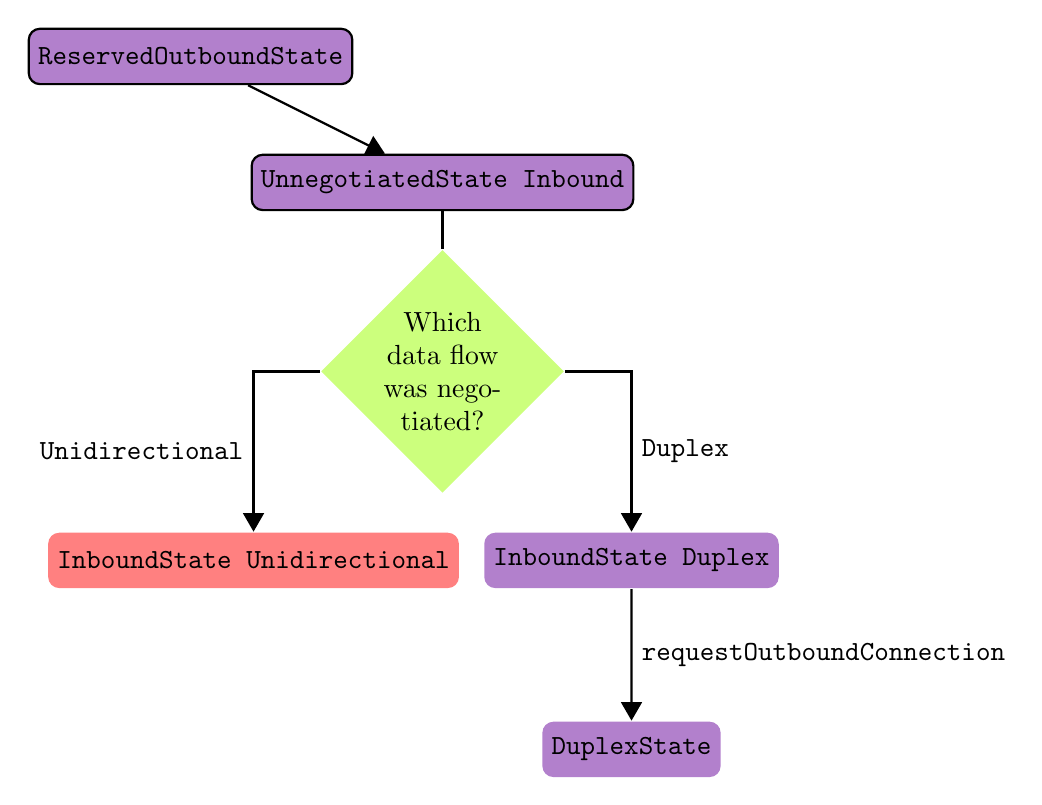
\begin{tikzpicture}[scale=0.8]
    \node[inbound_outbound_state,draw] (reserved_outbound)    at (-4, 0) {\ReservedOutboundState};
    \node[inbound_outbound_state,draw] (unnegotiated_inbound) at (0, -2)  {\UnnegotiatedStateIn};
    \draw[->] (reserved_outbound) -- (unnegotiated_inbound);

    \node[decision] (handshake_decision_inbound) at (0, -5) {Which data flow was negotiated?};
    \draw (unnegotiated_inbound) -- (handshake_decision_inbound);
    \node[inbound_state]          (inbound_unidf) at (-3, -8) {\InboundStateUni{}};
    \node[inbound_outbound_state] (inbound_dupdf) at (3,  -8) {\InboundStateDup{}};
    \draw[->] (handshake_decision_inbound.west) -| node[left, near end]{\textbf{\texttt{Unidirectional}}} (inbound_unidf);
    \draw[->] (handshake_decision_inbound.east) -| node[right,near end]{\textbf{\texttt{Duplex}}}         (inbound_dupdf);

    \node[inbound_outbound_state] (duplex) at (3, -11) {\DuplexState{}};
    \draw[->] (inbound_dupdf) -- node[right]{\textbf{\texttt{requestOutboundConnection}}} (duplex);
  \end{tikzpicture}}
  \caption{\textit{Inbound} connection flow graph, where both bordered states:
  \ReservedOutboundState{} and \UnnegotiatedStateIn are initial states.}
\end{figure}

\subsection{Server}

The server constists of two components: an accept loop and an \inbgov{}.  The
accept loop is using \texttt{includeInboundConnnection} on incoming
connections, while the \inbgov{} tracks the state of responder side of all
mini-protocols, and is responsible for starting and restarting mini-protocols
as well as detecting usage of them to support the \PromotedToWarmDupRem{}
transition and detecting termination to support the \DemotedToColdUniRem{}
transition.

The \inbgov{} will alway start / re-start all the mini-protocols using
\texttt{StartOnDemand} strategy.  When the multiplexer detects
any traffic on its ingress queues corresponding to responder protocols, the
\inbgov{} will schedule \PromotedToWarmDupRem{} transition with
\texttt{promotedToWarmRemote}.

We detect \DemotedToColdUniRem{} transition as soon as all respnder
mini-protocol are idle for a configurable delay (called
\texttt{serverRespondersIdleTimeout}).  One must use timeout, since it might
happen that a mini-protocol termination message arrives before initial message
of any other mini-protocols, for example when a connection starts and a node is
immediately promoted to \hot{} peer, it might happen that the termination message of
a \warm{} protocol (e.g. \tipSample{}) arrives before initial message of
the \keepAlive{} protcol.

Once \DemotedToColdUniRem{} transition is detected, the \inbgov{} will notify
the \connmngr{} using:

\begin{lstlisting}
-- | Returns 'True' if succeeds, 'False' if the connection is in 'Duplex'
-- state.
unregisterInboundConnection *'$\coloncolon$'* peerAddr *'$\Rightarrow$'* m (OperationResult Bool)
\end{lstlisting}
Which preforms either:
\begin{itemize}
  \item \DemotedToColdUniRem{}, or
  \item \DemotedToColdDupRem{} transition.
\end{itemize}
The first transition, as well as the case
\[
  \text{\DemotedToColdDupRem:\ \InboundStateDup{}}\rightarrow\text{\TerminatingState{}}
\]
will terminate the connection thread and call \texttt{close} the socket.
Though in this case the connection is unlikely to end in \texttt{TIME\_WAIT}
state, what happens in when a connection is reestablished might depend on the
implementation and sequence number of the initial \texttt{SYN}
packet\cite[Chapter 2, \texttt{TIME\_WAIT} section]{stevens2003unix}.

\subsubsection{Forceful termination}
The \connmngr{} might reset a connection through one of the \Prune{}
transitions.

\subsection{Inbound protocol governor in \texttt{ResponderMode}}
When the \connmngr{} runs in \texttt{ResponderMode} it will only expose
methods to make transition for inbound connections, i.e.
\texttt{includeInboundConnection} and \texttt{unregisterInboundConnection}.

In this case the connection state machine simplifies to:

\subsection{Connection manager methods}
\subsubsection{\texttt{includeInboundConnection}}
\begin{center}
  \begin{tabular}[h]{ll}
    \textit{State}           & \textit{Action} \\\hline\\[2pt]
    \InitialState{}          &
      \begin{minipage}[t]{8cm}
        \begin{itemize}
          \item start connection thread (handshake, \mux{})
          \item \NegotiatedUniIn{} or \NegotiatedDupIn{}
        \end{itemize}
      \end{minipage}
      \vspace{8pt}\\
    \ReservedOutboundState{} &
      \begin{minipage}[t]{8cm}
        \begin{itemize}
          \item \Overwritten{},
          \item start connection thread (handshake, \mux{})
          \item \NegotiatedUniIn{} or \NegotiatedDupIn{}
        \end{itemize}
      \end{minipage}
      \vspace{8pt}\\
    \UnnegotiatedStateAny{}  & \texttt{impossible state} \\[8pt]
    \OutboundStateAny{}      & \texttt{impossible state} \\[8pt]
    \DuplexState{}           & \texttt{impossible state} \\[8pt]
    \InboundStateAny{}       & \texttt{impossible state} \\[8pt]
    \TerminatingState{}      & the same as \InitialState{} \\[8pt]
    \TerminatedState{}       & the same as \InitialState{} \\[8pt]
  \end{tabular}
\end{center}

\subsection{\texttt{unregisterInboundConnection}}
\begin{center}
  \begin{tabular}[h]{lll}
    \textit{State}           & \textit{Action} & \textit{Returned Value}\\\hline\\[2pt]
    \InitialState{}          & \texttt{no-op} & \True \\[8pt]
    \ReservedOutboundState{} & error \texttt{ForbiddenOperation} & - \\[8pt]
    \UnnegotiatedStateAny{}  & error \texttt{ForbiddenOperation} & - \\[8pt]
    \OutboundStateAny{}      & error \texttt{ForbiddenOperation} & - \\[8pt]
    \DuplexState{}           & \DemotedToColdDupRem{}            & \False \\[8pt]
    \InboundStateUni{}       & transition to \TerminatedState{}  & \True \\[8pt]
    \InboundStateDup{}       & transition to \TerminatingState{} & \False \\[8pt]
    \TerminatingState{}      & error \texttt{ForbiddenOperation} & - \\[8pt]
    \TerminatedState{}       & error \texttt{ForbiddenOperation} & - \\[8pt]
  \end{tabular}
\end{center}

\subsection{\texttt{promotedToWarmRemote}}
\begin{center}
  \begin{tabular}[h]{lll}
    \textit{StateIn}         & \textit{StateOut}\\\hline\\[2pt]
    \InitialState{}          & \InitialState{}          \\[8pt]
    \ReservedOutboundState{} & \ReservedOutboundState{} \\[8pt]
    \UnnegotiatedStateAny{}  & \UnnegotiatedStateAny{}  \\[8pt]
    \OutboundStateUni{}      & \OutboundStateUni{}      \\[8pt]
    \OutboundStateDup{}      & \DuplexState{}           \\[8pt]
    \DuplexState{}           & \DuplexState{}           \\[8pt]
    \InboundStateUni{}       & \InboundStateUni{}       \\[8pt]
    \InboundStateDup{}       & \InboundStateDup{}       \\[8pt]
    \TerminatingState{}      & \TerminatingState{}      \\[8pt]
    \TerminatedState{}       & \TerminatedState{}       \\[8pt]
  \end{tabular}
\end{center}
The implmentation might use this method when an established mini-protocol
received a message as a method of detection of remote state transition.  Even
though we currently have only one established mini-protocol (i.e. \textit{keep
alive protocol}),  this method should be idempotent.

\bibliographystyle{abbrv}
\bibliography{connection-manager}
\end{document}
